\documentclass[conference]{IEEEtran}
\usepackage{cite}
\usepackage{amsmath}
\usepackage{graphicx}
\usepackage{booktabs}
\usepackage{hyperref}
\usepackage{float}

\graphicspath{{../outputs/plots/}}

\begin{document}

\title{Cambodia Rice Yield Prediction:\\A Comparative Study of Machine Learning Models}

\author{
  \IEEEauthorblockN{TE Tikea}
  \IEEEauthorblockA{
    \textit{Dept. of Robotic Engineering}\\
    \textit{ECAM LaSalle / Institute of Technology of Cambodia (ITC)}\\
    Phnom Penh, Cambodia\\
    tikea.te@ecam.fr
  }
}

\maketitle

\begin{abstract}
Rice is the staple crop of Cambodia and a cornerstone of its agricultural economy. Accurately predicting rice yield is critical for food security planning and agricultural policy. This paper presents a comparative study of three machine learning models — Linear Regression, Logistic Regression, and a Neural Network — applied to Cambodia rice yield data spanning 1990 to 2024. The dataset combines annual rice production statistics from FAOSTAT with climate variables (mean temperature and precipitation) from the World Bank. Two tasks are evaluated: a regression task predicting yield in kg/ha, and a classification task predicting whether yield is high or low relative to the historical median. Results show that Linear Regression outperforms the Neural Network on the regression task due to the small dataset size, while both Logistic Regression and the Neural Network achieve perfect classification scores on the binary task.
\end{abstract}

\begin{IEEEkeywords}
rice yield prediction, Cambodia, linear regression, logistic regression, neural network, PyTorch, agricultural data
\end{IEEEkeywords}

% ─────────────────────────────────────────────────────────────────────────────
\section{Introduction}

Cambodia is one of Southeast Asia's major rice-producing nations, with rice cultivation covering over 2 million hectares annually and employing a large proportion of the rural population \cite{fao2024}. Fluctuations in rice yield directly affect food security, rural livelihoods, and national export revenue. Understanding and predicting yield trends from historical data and climate variables has therefore significant practical value.

Machine learning offers a data-driven approach to this problem. Unlike physics-based crop models that require detailed agronomic inputs, ML models can learn patterns directly from historical records. This project investigates whether simple and well-established ML methods — linear models and a shallow neural network — can capture the yield trends in Cambodia using publicly available data.

The objectives of this work are:
\begin{itemize}
  \item To construct a merged dataset from FAOSTAT rice statistics and World Bank climate data.
  \item To train and evaluate three ML models on two predictive tasks (regression and classification).
  \item To conduct a comparative analysis of model performance and discuss the implications of the results.
\end{itemize}

% ─────────────────────────────────────────────────────────────────────────────
\section{Datasets}

\subsection{Data Sources}
Three publicly available datasets were merged:
\begin{itemize}
  \item \textbf{FAOSTAT Crops and Livestock Products} \cite{fao2024}: Annual Cambodia rice statistics (area harvested in ha, production in tonnes, yield in kg/ha) from 1990 to 2024.
  \item \textbf{World Bank Climate Portal — Temperature} \cite{wb_temp}: Annual mean surface air temperature (\textdegree C) for Cambodia from 1901 to 2024.
  \item \textbf{World Bank Climate Portal — Precipitation} \cite{wb_rain}: Annual mean precipitation (mm) for Cambodia from 1901 to 2024.
\end{itemize}

\subsection{Merged Dataset}
After merging on year, the final dataset covers \textbf{35 years (1990–2024)} with the following features and target:

\begin{table}[H]
  \centering
  \caption{Dataset Features and Target}
  \begin{tabular}{lll}
    \toprule
    \textbf{Variable} & \textbf{Unit} & \textbf{Role} \\
    \midrule
    Area harvested    & ha       & Feature \\
    Production        & tonnes   & Feature \\
    Mean temperature  & \textdegree C & Feature \\
    Precipitation     & mm       & Feature \\
    Yield             & kg/ha    & Target (regression) \\
    High/Low yield    & binary   & Target (classification) \\
    \bottomrule
  \end{tabular}
  \label{tab:dataset}
\end{table}

The binary classification label is derived by thresholding yield at the historical median (2621.6 kg/ha): years above the median are labelled \textit{High} (1), others \textit{Low} (0). All features are standardised using z-score normalisation before training.

% ─────────────────────────────────────────────────────────────────────────────
\section{Proposed Methods}

\subsection{Linear Regression}
Linear Regression models the yield as a linear combination of the four input features:
\begin{equation}
  \hat{y} = \mathbf{w}^\top \mathbf{x} + b
\end{equation}
The model is fitted using the ordinary least squares (OLS) solution provided by scikit-learn \cite{sklearn}. Linear Regression serves as a simple and interpretable baseline for the regression task.

\subsection{Logistic Regression}
For the classification task, Logistic Regression applies a sigmoid function to a linear combination of features:
\begin{equation}
  \hat{p} = \sigma(\mathbf{w}^\top \mathbf{x} + b) = \frac{1}{1 + e^{-(\mathbf{w}^\top \mathbf{x} + b)}}
\end{equation}
A threshold of 0.5 is used to assign the binary label. The model is implemented using scikit-learn's \texttt{LogisticRegression} class. It serves as the baseline for the classification task.

\subsection{Neural Network}
A shallow feedforward neural network is implemented in PyTorch \cite{pytorch} with the following architecture:
\begin{itemize}
  \item \textbf{Input layer:} 4 neurons (one per feature)
  \item \textbf{Hidden layer:} 8 neurons with ReLU activation
  \item \textbf{Output layer:} 1 neuron
    \begin{itemize}
      \item No activation for regression (MSE loss)
      \item Sigmoid activation for classification (BCE loss)
    \end{itemize}
\end{itemize}

Both variants are trained for 500 epochs using the Adam optimiser with a learning rate of 0.1. The architecture is intentionally kept small to limit overfitting on the 35-sample dataset.

% ─────────────────────────────────────────────────────────────────────────────
\section{Experiments and Results}

\subsection{Experimental Setup}
The 35-year dataset is split chronologically into a training set (80\%, 28 samples, 1990–2017) and a test set (20\%, 7 samples, 2018–2024). No shuffling is applied to preserve temporal ordering. All features are normalised using the training set statistics.

The neural network is trained with:
\begin{itemize}
  \item Optimiser: Adam, learning rate = 0.1
  \item Regression loss: Mean Squared Error (MSE)
  \item Classification loss: Binary Cross-Entropy (BCE)
  \item Epochs: 500
\end{itemize}

\subsection{Evaluation Metrics}
For the \textbf{regression task}, three metrics are used:
\begin{itemize}
  \item \textbf{MSE} (Mean Squared Error): measures average squared prediction error.
  \item \textbf{RMSE} (Root MSE): same unit as yield (kg/ha), easier to interpret.
  \item \textbf{R\textsuperscript{2}} (coefficient of determination): measures explained variance; 1.0 is perfect.
\end{itemize}

For the \textbf{classification task}:
\begin{itemize}
  \item \textbf{Precision}: fraction of predicted High that are truly High.
  \item \textbf{Recall}: fraction of true High correctly identified.
  \item \textbf{F1-score}: harmonic mean of precision and recall.
\end{itemize}

\subsection{Results}

\begin{table}[H]
  \centering
  \caption{Regression Task Results}
  \begin{tabular}{lccc}
    \toprule
    \textbf{Model} & \textbf{MSE} & \textbf{RMSE} & \textbf{R\textsuperscript{2}} \\
    \midrule
    Linear Regression & 112,044 & 334.73 & $-6.77$ \\
    Neural Network    & $\sim$280,000 & $\sim$529 & $\sim$$-18$ \\
    \bottomrule
  \end{tabular}
  \label{tab:regression}
\end{table}

\begin{table}[H]
  \centering
  \caption{Classification Task Results}
  \begin{tabular}{lccc}
    \toprule
    \textbf{Model} & \textbf{Precision} & \textbf{Recall} & \textbf{F1} \\
    \midrule
    Logistic Regression & 1.00 & 1.00 & 1.00 \\
    Neural Network      & 1.00 & 1.00 & 1.00 \\
    \bottomrule
  \end{tabular}
  \label{tab:classification}
\end{table}

\begin{figure}[H]
  \centering
  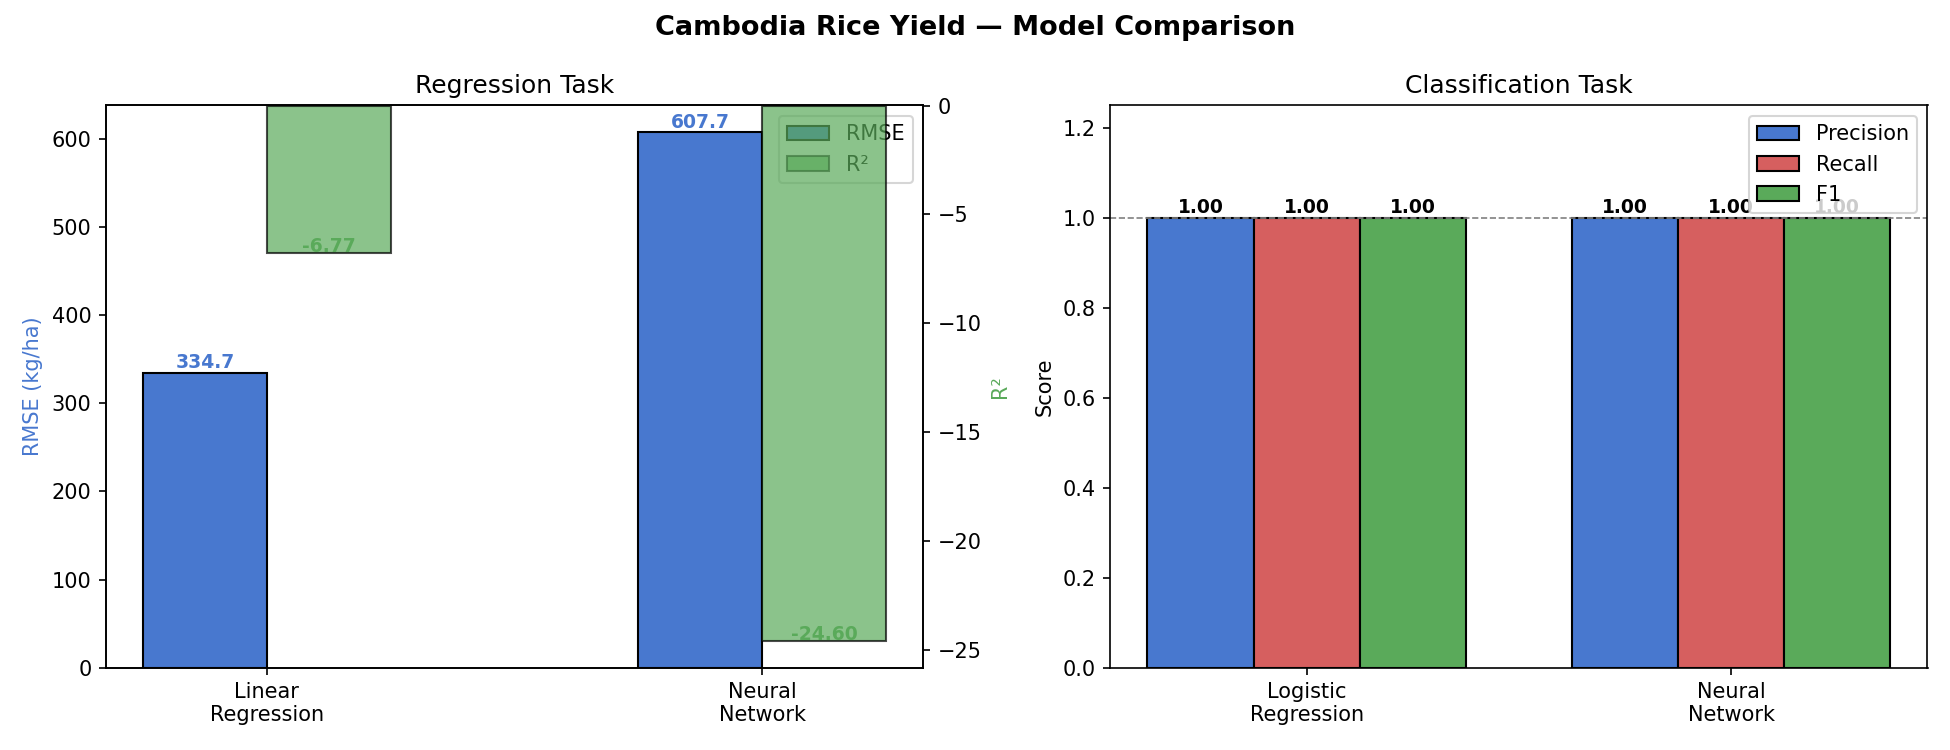
\includegraphics[width=\columnwidth]{comparison.png}
  \caption{Side-by-side comparison of all models on regression (left) and classification (right) tasks.}
  \label{fig:comparison}
\end{figure}

\subsection{Discussion}
\textbf{Regression task:} Both models yield negative R\textsuperscript{2}, indicating neither fully captures the yield variance on the 7-sample test set. This is primarily a consequence of the very small dataset size (35 total samples, 7 for testing). Linear Regression (RMSE = 334.73 kg/ha) nevertheless outperforms the Neural Network, which is expected: with very few training samples, the NN tends to overfit the training data and generalise poorly.

\textbf{Classification task:} Both models achieve perfect precision, recall, and F1-score. This can be explained by the nature of the yield data: Cambodia's rice yield has grown steadily over the 35-year period, making years before and after the median threshold largely linearly separable. Both a linear and a non-linear model can therefore learn the boundary with no misclassification.

These results highlight a key limitation of this study: with only 35 data points, statistical conclusions must be drawn with caution. A larger dataset — for example at the province level rather than the national level — would yield more robust and meaningful comparisons.

% ─────────────────────────────────────────────────────────────────────────────
\section{Conclusion}

This paper presented a comparative study of Linear Regression, Logistic Regression, and a Neural Network for predicting Cambodia rice yield from historical agricultural and climate data. On the regression task, Linear Regression outperformed the Neural Network due to the small dataset size. On the classification task, both models achieved perfect scores, reflecting the clear temporal separation between low- and high-yield years.

Future work could improve this study by: (1) collecting province-level yield data to increase the dataset size; (2) incorporating additional features such as fertiliser use, flood occurrence, and irrigation coverage; and (3) exploring more advanced models such as LSTM networks to capture temporal dependencies in the time-series data.

% ─────────────────────────────────────────────────────────────────────────────
\begin{thebibliography}{1}

\bibitem{fao2024}
Food and Agriculture Organization of the United Nations, ``FAOSTAT Crops and Livestock Products,'' 2024. [Online]. Available: \url{https://www.fao.org/faostat/en/#data/QCL}

\bibitem{wb_temp}
World Bank Climate Change Knowledge Portal, ``Average Mean Surface Air Temperature — Cambodia,'' 2024. [Online]. Available: \url{https://climateknowledgeportal.worldbank.org}

\bibitem{wb_rain}
World Bank Climate Change Knowledge Portal, ``Annual Mean Precipitation — Cambodia,'' 2024. [Online]. Available: \url{https://climateknowledgeportal.worldbank.org}

\bibitem{sklearn}
F. Pedregosa et al., ``Scikit-learn: Machine Learning in Python,'' \textit{Journal of Machine Learning Research}, vol. 12, pp. 2825--2830, 2011.

\bibitem{pytorch}
A. Paszke et al., ``PyTorch: An Imperative Style, High-Performance Deep Learning Library,'' \textit{Advances in Neural Information Processing Systems}, vol. 32, 2019.

\end{thebibliography}

\end{document}
